% !TEX TS-program = pdflatex
% !TEX encoding = UTF-8 Unicode

% This is a simple template for a LaTeX document using the "article" class.
% See "book", "report", "letter" for other types of document.

\documentclass[11pt, preview]{standalone} % use larger type; default would be 10pt

\usepackage[utf8]{inputenc} % set input encoding (not needed with XeLaTeX)


\usepackage{../../markup}
%%% Examples of Article customizations
% These packages are optional, depending whether you want the features they provide.
% See the LaTeX Companion or other references for full information.

%%% PAGE DIMENSIONS
\usepackage{geometry} % to change the page dimensions
\geometry{a4paper} % or letterpaper (US) or a5paper or....
% \geometry{margin=2in} % for example, change the margins to 2 inches all round
% \geometry{landscape} % set up the page for landscape
%   read geometry.pdf for detailed page layout information

\usepackage{graphicx} % support the \includegraphics command and options
\usepackage{color, tikz}
% \usepackage[parfill]{parskip} % Activate to begin paragraphs with an empty line rather than an indent

%%% PACKAGES
\usepackage{amsmath, amsfonts,amssymb}
\usepackage{booktabs} % for much better looking tables
\usepackage{array} % for better arrays (eg matrices) in maths
\usepackage{paralist} % very flexible & customisable lists (eg. enumerate/itemize, etc.)
\usepackage{verbatim} % adds environment for commenting out blocks of text & for better verbatim
\usepackage{subfig} % make it possible to include more than one captioned figure/table in a single float
% These packages are all incorporated in the memoir class to one degree or another...

%%% HEADERS & FOOTERS
\usepackage{fancyhdr} % This should be set AFTER setting up the page geometry
\pagestyle{fancy} % options: empty , plain , fancy
\renewcommand{\headrulewidth}{0pt} % customise the layout...
\lhead{}\chead{}\rhead{}
\lfoot{}\cfoot{\thepage}\rfoot{}

%%% SECTION TITLE APPEARANCE
\usepackage{sectsty}
\allsectionsfont{\sffamily\mdseries\upshape} % (See the fntguide.pdf for font help)
% (This matches ConTeXt defaults)

%%% ToC (table of contents) APPEARANCE
\usepackage[nottoc,notlof,notlot]{tocbibind} % Put the bibliography in the ToC
\usepackage[titles,subfigure]{tocloft} % Alter the style of the Table of Contents
\renewcommand{\cftsecfont}{\rmfamily\mdseries\upshape}
\renewcommand{\cftsecpagefont}{\rmfamily\mdseries\upshape} % No bold!

\newcommand{\N}{\mathbb{N}}
\newcommand{\Prob}{\mathbb{P}}
\newcommand{\E}{\mathbb{E}}
\newcommand{\Z}{\mathbb{Z}}
\newcommand{\R}{\mathbb{R}}
\newcommand{\Q}{\mathbb{Q}}
%%% END Article customizations

%%% The "real" document content comes below...

\date{} % Activate to display a given date or no date (if empty),
         % otherwise the current date is printed 

\begin{document}
\config{name}{Random Variables and Probability Distributions}
\noindent{\bf Random Variables and Probability Distributions.}

\begin{enumerate}
\item {\bf Random Variables.} Consider the following game: you roll two standard 6-sided dice, one after the other. If the number on the first dice divides the number on the second dice, you get 1 point. You get 1 additional point for each prime number you roll.

Define the random variable $R_1$ to be the result of the first roll, and define $R_2$ to be the result of the second roll. Define the random variable $X = R_1 + R_2$ to be the sum of the numbers that come up on both dice, define the random variable $Y = R_1 \cdot R_2$ to be the product of the numbers that come up on both dice, and define the random variable $Z$ to be the number of points you win in the game.

\begin{enumerate}
\item How many values can the random variable $Z$ take on (with nonzero probability)?
\begin{Freeform}{3}
\# values of $Z$ = 
\Hint What are all the possible values of $Z$ as it is defined in this game?
\end{Freeform}
%-----------------------------------------
\item What are the minimum and maximum values that the random variable $Z$ take on  (with nonzero probability)? Please enter your answer in the form $(x,y)$ where $x$ is the minimum value and $y$ is the maximum value (be sure not to use a space!).
\begin{Freeform}{(0,2)}
$(\min Z, \max Z)$ = 
\Hint What are all the possible values of $Z$ as it is defined in this game?
\end{Freeform}
%-----------------------------------------
\item Say that your first roll is a 3 and your second roll is a 6. What is the value of $Z$?
\begin{Freeform}{2}
$Z$ = 
\Hint Review the definition of a random variable--what is the value of this expression given the sample point?
\end{Freeform}
%-----------------------------------------
\item Say that your first roll is a 2 and your second roll is a 1. What is the value of $Z$?
\begin{Freeform}{1}
$Z$ = 
\Hint Review the definition of a random variable--what is the value of this expression given the sample point?
\end{Freeform}
%-----------------------------------------
\item Say that your first roll is a 4 and your second roll is a 1. What is the value of $X^2+Y$?
\begin{Freeform}{29}
$X^2+Y$ = 
\Hint Review the definition of a random variable--what is the value of this expression given the sample point?
\end{Freeform}
%-----------------------------------------
\item Say that your first roll is a 3 and your second roll is a 5. What is the value of $X+Y+2\cdot Z$?
\begin{Freeform}{27}
$X+Y+2\cdot Z$ = 
\Hint Review the definition of a random variable--what is the value of this expression given the sample point?
\end{Freeform}
%-----------------------------------------
\item Conditioned on the fact that your second roll is a 1, what is the probability that $Z = 1$? Please enter your answer as a completely reduced fraction (i.e. in the form $x/y$ where $x,y$ are the smallest possible non-negative integers).
\begin{Freeform}{2/3}
$\Prob[Z = 1|R_2 = 1]$ = 
\Hint Review the definition of a random variable--on how many sample points in the event we are conditioning on does $Z$ take value $1$?
\end{Freeform}
%-----------------------------------------
\item Conditioned on the fact that your second roll is a 1, what is the probability that $Z = 2$?  Please enter your answer as a completely reduced fraction (i.e. in the form $x/y$ where $x,y$ are the smallest possible non-negative integers).
\begin{Freeform}{0/1}
$\Prob[Z = 2 | R_2 = 1]$ = 
\Hint Review the definition of a random variable--on how many sample points in the event we are conditioning on does $Z$ take value $2$?
\end{Freeform}
%-----------------------------------------
\end{enumerate}
%---------------------------------------------------------------------------------------------------------
\item {\bf Distributions of Random Variables.} Match each of the 5 random variables below with the correct probability distribution (of the following choices):

\begin{center}
\begin{tabular}{c|c}
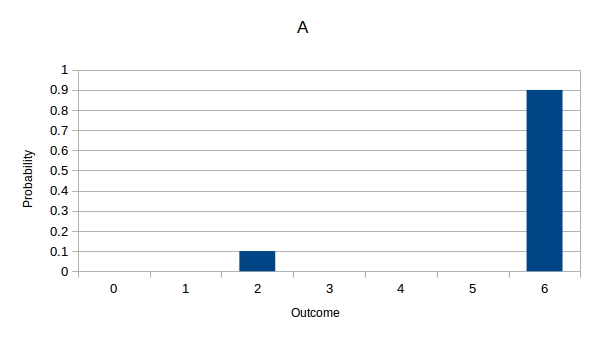
\includegraphics[width=0.4\textwidth]{dists/candy.png} &
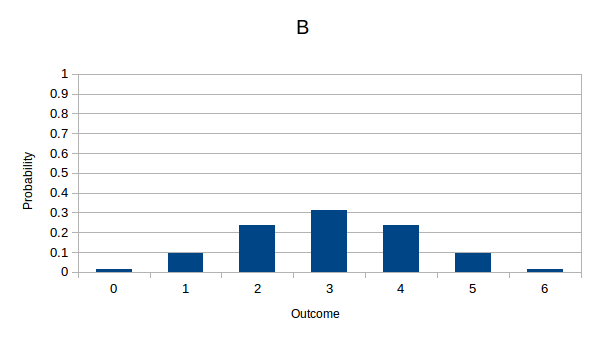
\includegraphics[width=0.4\textwidth]{dists/binom.png}
\\
\hline 
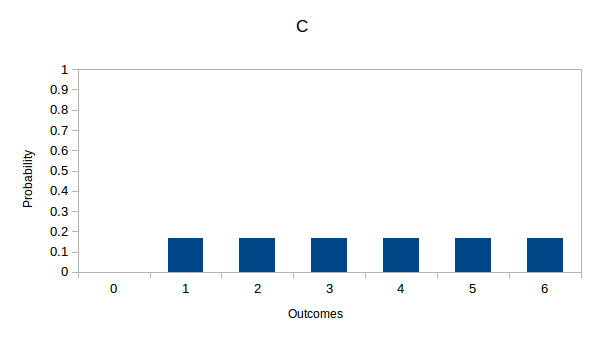
\includegraphics[width=0.4\textwidth]{dists/uniform.png}&
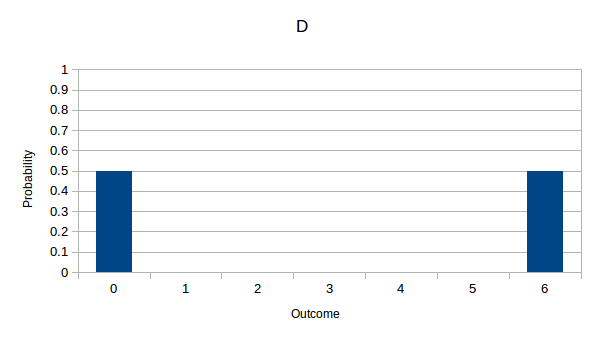
\includegraphics[width=0.4\textwidth]{dists/extreme.png}\\
\hline \vspace{2mm}
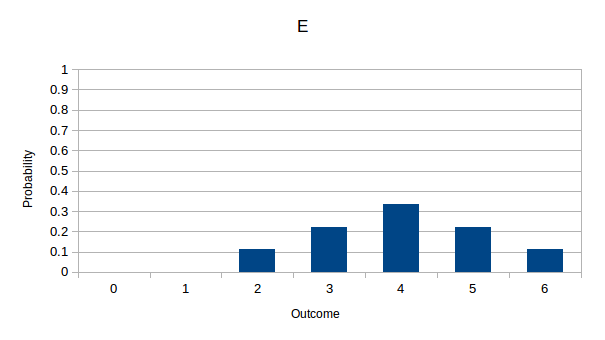
\includegraphics[width=0.4\textwidth]{dists/twodice.png}&
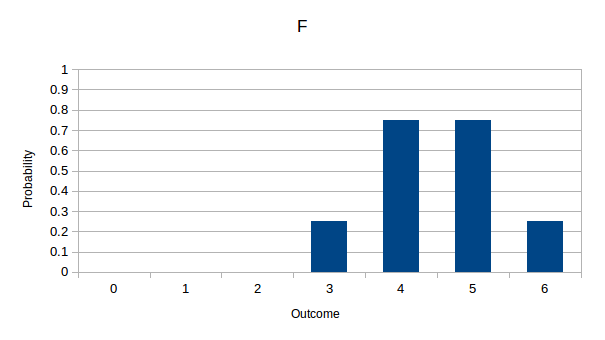
\includegraphics[width=0.4\textwidth]{dists/threeflips.png}\\
\end{tabular}
\end{center}

\begin{enumerate}
%-----------------------------------
\item What is the distribution corresponding to the number of tails, $X$, generated in 6 coinflips?
\begin{Multi}
Review the definition of a random variable and the definition of a probability distribution in note 12.
\begin{itemize}
\FalseChoice\item A
\TrueChoice\item B
\FalseChoice\item C
\FalseChoice\item D
\FalseChoice\item E
\FalseChoice\item F
\end{itemize}
\end{Multi}
%-----------------------------------
\item  What is the distribution corresponding to the outcome $X$ of rolling a standard 6-sided dice?
\begin{Multi}
Review the definition of a random variable and the definition of a probability distribution in note 12.
\begin{itemize}
\FalseChoice\item A
\FalseChoice\item B
\TrueChoice\item C
\FalseChoice\item D
\FalseChoice\item E
\FalseChoice\item F
\end{itemize}
\end{Multi}
%-----------------------------------
\item What is the distribution corresponding to the sum $X_1 + X_2$ of the outcomes of two 3-sided dice, each with sides labeled 1,2,3?
\begin{Multi}
Review the definition of a random variable and the definition of a probability distribution in note 12.
\begin{itemize}
\FalseChoice\item A
\FalseChoice\item B
\FalseChoice\item C
\FalseChoice\item D
\TrueChoice\item E
\FalseChoice\item F
\end{itemize}
\end{Multi}
%-----------------------------------
\item  What is the distribution corresponding to the sum $Z_1 + Z_2 + Z_3$, where $Z_i$ is generated by flipping a coin and setting $Z_i = 2$ if it turns up heads and $Z_i = 1$ if it turns up tails (or, if you like, the sum of three 2-sided dice)?
\begin{Multi}
Review the definition of a random variable and the definition of a probability distribution in note 12.
\begin{itemize}
\FalseChoice\item A
\FalseChoice\item B
\FalseChoice\item C
\FalseChoice\item D
\FalseChoice\item E
\TrueChoice\item F
\end{itemize}
\end{Multi}
%-----------------------------------
\item Say a candy bar is sold for $\$6$ at the corner store, but is sold for $\$2$ at the MegaMart one mile away. Because the MegaMart is 9 times further away than the corner store, you are 9 times more likely to buy the candy bar at the corner store.  What is the distribution corresponding to the price $X$ you pay for the candy bar on a random day (assuming you choose randomly whether to go to the corner store or the MegaMart with probability proportional to the distance).
\begin{Multi}
Review the definition of a random variable and the definition of a probability distribution in note 12.
\begin{itemize}
\TrueChoice\item A
\FalseChoice\item B
\FalseChoice\item C
\FalseChoice\item D
\FalseChoice\item E
\FalseChoice\item F 
\end{itemize}
\end{Multi}
%-----------------------------------
\item When it rains it pours--say that this past April, on half of the days of April there were 0 inches of rain, and the other half of the days there were 6 inches of rain. What is the distribution of $X$, the number of inches of rain on a uniformly random day of April?  
\begin{Multi}
Review the definition of a random variable and the definition of a probability distribution in note 12.
\begin{itemize}
\FalseChoice\item A
\FalseChoice\item B
\FalseChoice\item C
\TrueChoice\item D
\FalseChoice\item E
\FalseChoice\item F
\end{itemize}
\end{Multi}
%-----------------------------------
\end{enumerate}
%---------------------------------------------------------------------------------------------------------
\item {\bf A Preview of Expectations.} Consider a random variable $X$ which takes on values $x_1, \ldots, x_n$. The \emph{expectation} of $X$, denoted $\E[X]$, is defined to be 
\[
\E[X] = \sum_{i = 1}^n x_i \cdot \Prob[X = x_i].
\]
Notice that when $\Prob[X = x_i] = \frac{1}{n}$ for all $i$, then this is simply the familiar notion of an average! You will learn more about the expectation next week, and you can refer to note 12 for more details. For now, we will practice calculating some expectations.

Let us return to the game from the first question: roll two 6-sided dice, award 1 point if the number on the first dice divides the number on the second dice, plus one more point for each prime. Define $R_1$ to be the result of the first roll, define $R_2$ to be the result of the second roll, define $X = R_1 + R_2$ to be the sum of the numbers that come up on both dice, define $Y = R_1 \cdot R_2$ to be the product of the numbers that come up on both dice, and define $Z$ to be the number of points you win in the game.
\begin{enumerate}
\item What is $\E[R_1]$?
\begin{Freeform}{3.5}
$\E[R_1]$ = 
\Hint Review the definition of expectation.
\end{Freeform}
%-----------------------------------------
\item What is $\E[X] = \E[R_1 + R_2]$?
\begin{Freeform}{7}
$\E[X]$ = 
\Hint Review the definition of expectation.
\end{Freeform}
%-----------------------------------------
\item What is $\E[2\cdot R_1]$? What do you notice about this expectation?
\begin{Freeform}{7}
$\E[X]$ = 
\Hint Review the definition of expectation.
\end{Freeform}
%-----------------------------------------
\item What is $\E[Z | R_2 = 1]$, the expected number of points we win conditioned on the fact that the second dice roll is a 1? Please enter your answer as a completely reduced fraction (i.e. in the form $x/y$ where $x,y$ are the smallest possible positive integers).
\begin{Freeform}{2/3}
$\E[Z | R_2 = 1]$ = 
\Hint Review the definition of expectation--here, we are only considering expectation over the sample points in which $R_2 = 1$.
\end{Freeform}
%-----------------------------------------
\end{enumerate}

\end{enumerate}
\end{document}
